\section{Introduction}
 The Next Release Problem(NRP) is the choice of what requirements the company will reflect when making the next version of the product. This problem is primarily aimed at helping the company get the most profit from limited costs. However, most of the previous studies were using random variables, not actual data values. 
 
 The reason is that first of all, it's quite difficult to define the cost and the profit. Cost and profits are quite difficult to quantify. Both have to be calculated before the actual requirements are applied, so we have to use estimates value, rather than actual values. The second reason is that the requirements for the company's next production are highly secured data to the company and are very difficult to use in real research. Even if your company provides data, the actual results are prohibited to open, and this often results in post-processing after the release.
 
 We point out that these processes are wrong. The real NRP is that the cost and profit are not independent, and because it is used in the real industry, the process of obtaining the cost and profit has to be included to entire process. Also, importing and writing data from the future makes it difficult for research results to be applied to actual industrial sites. So we chose our topic to build our own industrial data and apply search-based algorithms. 
 
Section 2 introduces the related paper about our topic. Section 3 introduces the basic model of the NRP problem that we are currently dealing with in our report.

We divided the main part of the report into two parts. First, in section 4, we will organize the requirements in the actual product and create a dataset. And in this process, we're not going to use any random variables, and we're not going to bring in actual profit and cost from the future. 
And in Section 5, we're going to apply different search-based algorithms to the datasets that we've created. In addition to SA, GA, and NSGA2, we also implemented ILP and AHP directly and applied them to datasets. We will apply them to actual datasets and compare the performance of each algorithm in terms of time cost and optimization answers. And we'll also see how much search-based algorithm has increased the profit compared to the actual true value.

All codes used in the paper can be found at 

https://github.com/shkevinlee/CS454

\section{Related Work}
The Next Release Problem(NRP)\cite{NRP} was proposed by Bagnall et al in 2001. In this paper, authors considered requirements which can be dependent on other requirements. And also, they set the importance(or weight) of each customer who demands for resolving requirements to company. They applied several heuristic method(various versions of simulated annealing and hill climbers) and concluded that the simulated annealing algorithm found the best solutions using only modes amounts of computing time in their dataset.

In the Multi-Objective Next Release Problem(MONRP)\cite{MONRP}, authors tried to solve this problem as the multi-objective optimization problem. They applied algorithms(Pareto GA, Single-objective GA, and NSGA-II) and concluded that the NSGA-II is well suited to the MONRP.

After these papers, there are many trials to select the optimal set of requirements.\cite{ILP} \cite{DE} \cite{ACO} However, in almost cases, they used the data set which is randomly generated.

Tonella et al. were applied the Interactive Genetic Algorithm and AHP to the NRP and requirements prioritization for real software system as part of the project ACube, but their constraint was number of information about the priority graph, not the limited budget.\cite{IGA} 



\section{The Model}

Let $R = \{r_1, r_2, \ldots, r_N\}$ is a set of all possible N requirements for software or company and each requirement $r_i \in R$ has its cost and profit, $cost_i \in \mathbb{Z}^+$ and $profit_i \in \mathbb{Z}^+$, to be performed. The cost is whatever company have to pay to resolve requirements, for example, money, time and etc. The profit is whatever company get by resolving requirements, for example, user satisfaction. In this project, we assumed that all requirements are independent. It means, there is no prerequisite of requirements. The cost vector $Cost$ and the profit vector $Profit$ for requirements are denoted by 
\[
Cost = \{cost_1, cost_2, \ldots, cost_N\}
\]
\[
Profit = \{profit_1, profit_2, \ldots, profit_N\}
\]

The company always wants to select requirements for the next release to get the highest sum of profits in the limited budget. Let the decision vector $\textbf{x} = \{x_1, x_2, \ldots, x_n\} \in \{0, 1\}$ where $x_i$ is 1 if requirement $i$ is selected and 0 otherwise. Then our objective function can be written as below:
\[
maximize \sum_{i = 1}^{N} profit_i \cdot x_i
\]
subject to
\[
\sum_{i = 1}^{N} cost_i \cdot x_i \leq B
\]
for some bound $B \in \mathbb{Z}^+$ which represents the limited budget.

\section{Data sets}
We tried to implement a dataset in the real industry.

\subsection{Bugzilla}

We chose Bugzilla where we could get the data source. 

Bugzilla is a web-based, general purpose bug tracker and test tool originally developed and used by the Mozilla project. When users or developers report bugs to the repository for each project in Bugzilla, the project manager or the developer in charge identifies them, reflects them on the product, or re-prioritizes them.

The biggest reason for choosing Bugzilla is that all the data is open. The actual requirements normally are not disclosed for security reasons. However, all the data is open because Bugzilla has to report on the bug. It also contains a number of data that can be used to estimates the cost and profit. The most recent version was announced in the 15th year, and many open sources, including the Mozilla Project, are actively using bug tracking.

Here are some of the Bugzilla sites in operation.

\textbf{Mozilla} -\textit{https://bugzilla.mozilla.org/}

\textbf{Eclipse} -\textit{ https://bugs.eclipse.org/bugs/}

We can assume that one bug is a requirement. And once you've solved this bug report, you can think of it as reflected in the next version.

\subsection{Open Source repository}

Now many open sources are actively using Bugzilla. We chose two of the most famous open sources, Firefox and Eclipse. Each repository consists of several platforms inside the open source. We decided to extract data from the two platforms where the most bugs were resolved in 2017. The \textbf{Firefox Web browser} platform was selected in the Firefox repository, and the \textbf{Eclipse platform} was selected in the Eclipse repository.


\subsection{Crawling Modeling}

We decided to create a dataset based on data from 2017. The reason is that if too many previous years of data are used, unresolved bugs are more likely to be reported incorrectly or missing than being pushed out of the priority list. Also, for real value comparison, we  needed some time to solve the bug, so we targeted 2017.

It's a little bit difficult to apply them right into the NRP problem because they're being reflected in the product in real time deployment. So we extract the data set based on a few assumptions:

\textbf{Requirements for 2017} : 2017. 1. 1. 00:00 to 2017. 12. 31 59:59 The issues registered in 2017 but not resolved shall be considered as requirements for products.

\textbf{Bugs Resolved in 2018 (true value)}: In the 2017 requirement, they are considered to be the requirements reflected in the next version of the actual product are considered.

The results of our target project are as follows table1
\begin{table} [H]
  \caption{Number of requirements}
  \label{tab:commands}
  \begin{tabular}{cccccl}
    \toprule
    &ECLIPSE PLATFORM&FIREFOX BROWSER\\
    \midrule
    Reported in 2017& 2053 & 5593 \\
    Resolved in 2018 & 817 & 2938 \\
    \bottomrule
  \end{tabular}
\label{table:Dataset}
\end{table}


\subsection{Research Question}

We're trying to extract the estimated cost and profit values from the crawled dataset. Our research question about dataset can be divided into two main areas.

\textbf{RQ1}. \textit{Could we estimate PROFIT from Bugzilla without Forward Looking?}

\textbf{RQ2}. \textit{Could we estimate COST from Bugzilla without Forward Looking?}

\begin{figure*}
\centering
  \begin{subfigure}[b]{0.45\linewidth}
    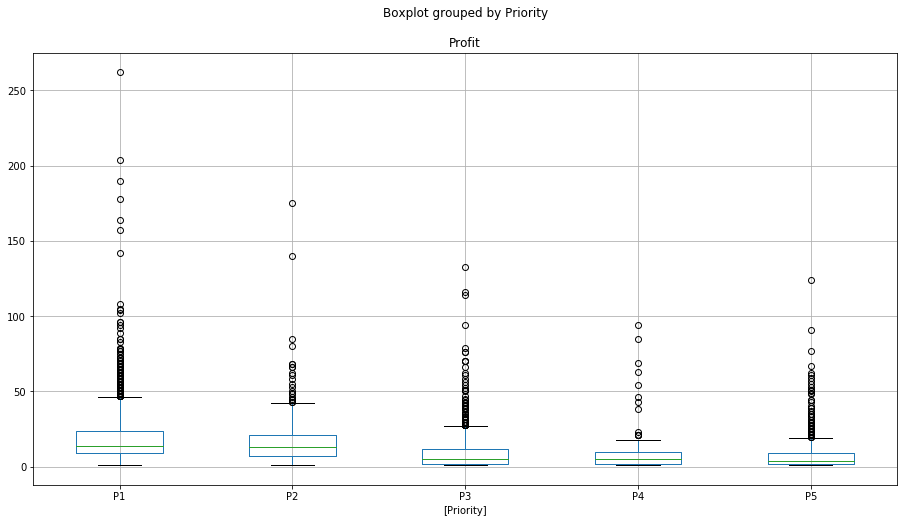
\includegraphics[width=\linewidth]{images/boxplotraw.png}
    \caption{Priority-number of comments}
  \end{subfigure}
  \begin{subfigure}[b]{0.45\linewidth}
    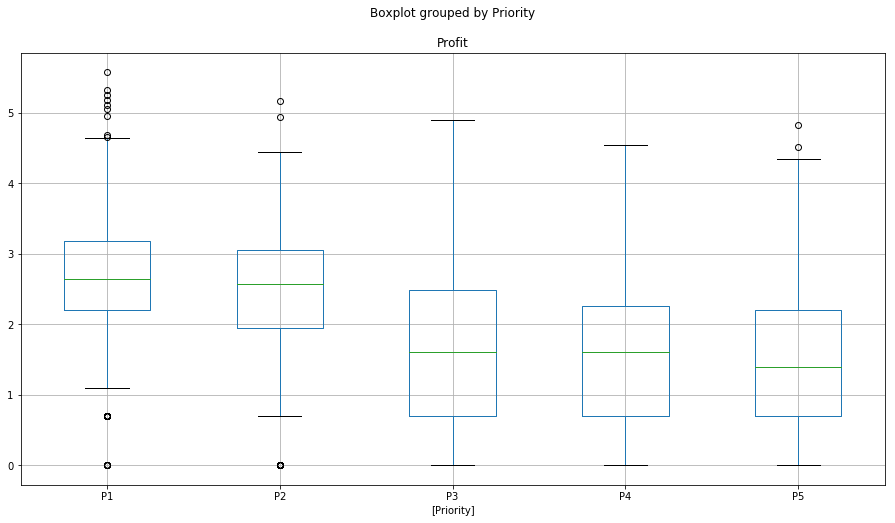
\includegraphics[width=\linewidth]{images/boxplot.png}
    \caption{Priority-Log(number of comments)}
  \end{subfigure}
  \caption{The relation ship between Priority and Number of Comments}
  \label{fig:priority_comments}
\end{figure*}
\begin{figure*}[h]
\centering
  \begin{subfigure}[b]{0.9\linewidth}
    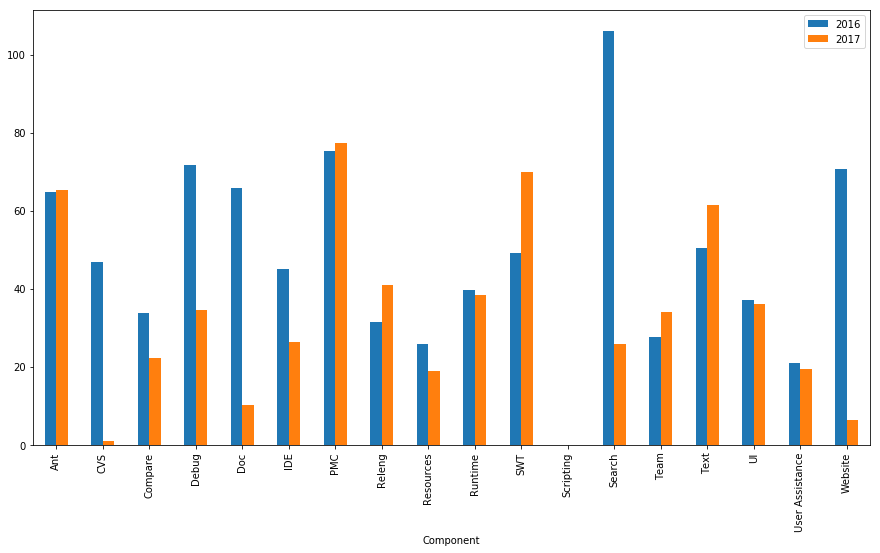
\includegraphics[width=\linewidth]{images/chart_ec.png}
    \caption{Eclipse}
  \end{subfigure}
  \begin{subfigure}[b]{0.9\linewidth}
    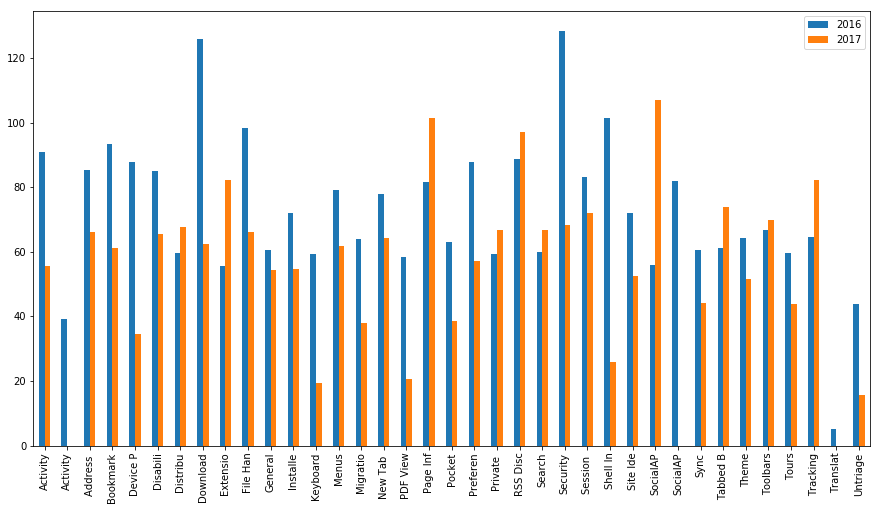
\includegraphics[width=\linewidth]{images/chart_ff.png}
    \caption{Firefox}
  \end{subfigure}
  \caption{Average Time cost at 2016 and 2017 per components}
  \label{fig:time_cost}
\end{figure*}
\subsection{Profit}

 Profit is an indicator of how much the value of the product has increased when the company has addressed this requirement. There were two indicators in Bugzilla that directly represented this value.
 
\textbf{Priority}: Priority for bugs

\textbf{Severity}: The Severity of the bug

And there are other indicators that show interest in bugs.


\textbf{Resolution, Votes, Number of Comments}


Among these, the indicators with sufficient coverage of the data were \textit{Priority} and \textit{Number of comments}. The rest of the indicators were either underutilized by the project manager, or there was not much value difference between the requirements. 

\textbf{Priority}: In the case of priority, the manager directly ranks the requirements, so it is also an accurate indicator of the profit. In the case of Bugzilla, they provide an interface to select Priority from a total of five stages, P1 to P5(P1 is the highest). The problem with Priority is that there is not much difference in values for each requirement because it is rank-based data. And because it's not a required metric, Eclipse has a lot of requirements that don't have priority entered, so it couldn't be used.


\textbf{Number of Comments}: An indicator of how much Discussion has occurred in the requirements. We assumed that the requirements would have a high priority if Discussion had occurred in those requirements.

 To find out, we compared the actual Priority to the Number of Comments. Figure 1.(a) shows this as a box plot. The higher the priority, the more the comment. However, you can see that there are too many outliers and that the data is distributed asymmetrically. This is because the number of comments follows a log distribution. So we applied the logarithmic function to the number of commands and then we compared it again. This is shown in Figure 1.(b) 

As Figure 1.(b) shows, Priority and Member of Comments have a linear relationship. Unlike Priority, Number of segments has a constant distribution of values and various values by requirement. Number of Comments is better than Priority to apply the actual search-based algorithm. 

\textbf{RQ1}.\textit{ Could we estimate PROFIT from Bugzilla without Forward Looking?}

We have concluded that we can speculate on Profit. Based on the manager's thinking priority and interest in this requirements, we were able to derive values for the profit between 1 and 5. Of course there are limitations. Number of comments is not a direct indicator, so exceptions must always be present. In addition, if the manager does not enter Priority, such as Eclipse repository, there is a significant lack of confidence in the value. If a priority index is entered forcibly, or if a more complex set of indicators such as the number of participants to discussion or number of views is considered, a more accurate profit can be drawn.


\subsection{Cost}

 Unlike Profit, the Cost was a very difficult task to figure out the actual prediction. In fact, it's very difficult for a product manager to calculate the time cost of a particular requirement, and the developers working on the actual task are just guessing how much time they'll take. 
 So we defined the Cost as: 
 
\textbf{Cost}: \textit{Average resolution time for the requirements of the same component as the previous year}

Bugzilla's repositories are divided into each component. We assumed that the average time it takes to fix the bug for each component would be a constant in next year. Therefore, We concluded that the average bug modification time for each component in 2017 would not be much different from 2016. So the Cost of each requirement was used as a prediction index for the average Cost of that component in 2016.

 To illustrate this, we compared the average time cost in 2016 to the average time cost in 2017. Figure 2 describes this.
 
As Figure 2.(a) shows, the first, the result in Eclipse repository is quite accurate. The average bug resolution time was similar than we expected. Some exceptions have been found to exist, but more than 60 percent of the components actually match.

But for Figure 2.(b) the result in Firefox repository, we can also see that the order of each component, including absolute time-consuming values, is not quite correct. In Firefox, it was updated almost 200 times a year. Therefore, in 2016 and 2017, the code was not maintained the same, so it make that the actual cost are not constant among the years. 

\textbf{RQ2}. \textit{Could we estimate COST from Bugzilla without Forward Looking?}

We have concluded that it is possible to use the past Cost only for projects where updates are infrequent, i.e. projects with some constant structure. This estimate process has many limitations to be used in real industry. It's a very change-sensitive indicator, and it has the potential to be wrong at any time. However, in order to estimate this more accurately, it would be the only way for the developer or project manager to specify the actual estimated time cost. In the absence of such direct data, our estimates will be meaningful.


\subsection{Result}

In conclusion, we were able to create 4 data sets. In Firefox, the profit was able to use both Priority and Number of Comments, creating a total of three data sets, including each case and the sum of the two indicators. The table also shows the true value of cost and profit that was resolved in 2018. We're going to use this dataset to compare the results of the actual search-based algorithms in the next section.

\begin{table} [H]
  \caption{Dataset from Bugzilla}
  \label{tab:commands}
  \begin{tabular}{cccccl}
    \toprule
    Repository&Profit definition&True Cost&True Profit\\
    % &ECLIPSE&FIREFOX-I&FIREFOX-II&FIREFOX-III\\
    \midrule
    ECLIPSE-I&Log(comments)&50699.70& 3489.64 \\
    FIREFOX-I&Log(comments)& 262945.50& 13025.8 \\
    FIREFOX-II&Priority& 262945.50& 12210 \\
    FIREFOX-III&Priority+Log(comments)& 262945.50& 26332.88 \\
    \bottomrule
  \end{tabular}
\label{table:Dataset}
\end{table}


\section{Algorithms}
We applied two deterministic algorithms(AHP and ILP) and three heuristic algorithms(SA, GA and NSGA-II) which were introduced as the algorithms well-suited for the NRP in papers\cite{NRP}\cite{ILP}\cite{IGA}\cite{MONRP}. And, to encourage the performance of heuristic algorithms, we put a greedy solution into the initial population or initial decision vector.

The greedy algorithm for the initial solution of heuristic algorithms is described as below. 

\begin{algorithm}
\caption{greedy algorithm}\label{alg:greedy}
\begin{algorithmic}
    \State Let $\textbf{x} = \{0, 0, \ldots, 0\}$ ;
    \State Let $CostSum = 0$ ;
    \For{$i = 1$ to $N$}
        \State $p = argmax(Profit)$ ;
        \If {$CostSum + cost_p \leq B$}
            \State $x_p = 1$ ;
            \State $CostSum = CostSum + cost_p$ ;
        \EndIf
        \State $profit_p = -\infty$ ;
    \EndFor
    \textbf{return} $x$
\end{algorithmic}
\end{algorithm}


\subsection{Analytic Hierarchy Process}
The Analytic Hierarchy Process(AHP) which was first applied to requirement prioritization by Karlsson and Ryan\cite{AHP} is a structured technique for organizing and analyzing complex decisions. To use the AHP for decision making in general, we had to perform pairwise comparisons of all the requirements to get their relative intensity. But, in our case, we don't have to compare relatively each other since each requirements has its own profit and cost. Therefore, we defined the relative intensity as the ratio of each requirement and made the profit-comparison matrix and the cost-comparison matrix by using them. And then, we calculated the priority vector. To get the optimal decision vector, we sorted the priority vector by its weight and selected requirements while the sum of costs didn't exceed the limited budget.


\subsection{Integer Linear Programming}
The Integer Linear Programming(ILP) is optimization method whose objective function and constraints are linear, and all variables are integer. The NRP can be treated as the ILP since each element of the decision vector $\textbf{x}$ is 0 or 1 and our constraint, the limited budget, is also linear. So we applied the ILP solver to the NRP problem.

Reference paper\cite{ILP} used ILP solver named \textit{CPLEX}, but it is commercial solver so we used \textit{PuLP}(modeler) and \textit{Gurobi}(solver) for this project. \textit{PuLP} is free open source software so users can use it. However, general \textit{Gurobi} solver is commercial one so we registered to \textit{Gurobi (www.gurobi.com)} and used \textit{Gurobi} academic version.

\subsection{Simulated Annealing}
Simulated annealing(SA) is one of the local search techniques which are iterative in nature and rely on the definition of a solution neighbourhood. For our NRP project, a requirement-based neighbourhood was defined. So the current solution can reach its neighbour by making small changes of decision vector $x$.

To apply the SA, we have to define a objective function to get the optimal decision vector:
\[
f(\textbf{x}) = \sum_{i = 1}^{N} profit_i \cdot x_i + \lambda \min \Big\{0, \sum_{i = 1}^{N} (cost_i \cdot x_i) - B \Big\}
\]
where $\textbf{x}$ is the decision vector, $f$ is our objective function and $\lambda$ is control parameter. We can impose a penalty if the sum of costs exceed the limited budget by using the control parameter $\lambda$. This objective function is also used in genetic algorithm to evaluate each chromosome.

In the NRP paper\cite{NRP}, the cooling schedule by Lundy and Mess\cite{LundySA} is well-suited. Their approach is presented below:
\[
    T_{i+1} = \frac{T_i}{1 + \beta T_i}
\]
where $T_i$ is the temperature at iteration $i$ and $\beta$ is control parameter. So for the Lundy and Mess cooling schedule, the temperature drops after each move.

The main loop of SA can be described in Algorithm \ref{alg:SA}. To increase the performance, we used a greedy solution as the initial decision vector. 

In our project, the parameter $\lambda$ and $\beta$ were set to 5 and $1 \times 10^{-8}$ since Bagnall et al. got the best solution for this value in their paper.


\begin{algorithm}
\caption{Simulated Annealing (SA)}\label{alg:SA}
\begin{algorithmic}
    \State $x \gets$ initial decision vector ;
    \State $T \gets$ initial temperature ; 
    \While{not stopping condition}
        \State $x_{new} \gets GetRandomNeigbour(x)$ ;
        \If {$AcceptanceRate(F(x), F(x_{new}), T) \geq random(0, 1)$}
            \State $x \gets x_{new}$ ;
        \EndIf
        \State $T \gets COOL(T)$ \Comment{Lundy and Mess}
    \EndWhile
    \textbf{return} $x$
\end{algorithmic}
\end{algorithm}

\subsection{Genetic Algorithm}
The Genetic Algorithm(GA) is one of the evolutionary algorithms. In our project, we used a single objective function for GA which is the same with the simulated annealing. To make offspring population, we used the tournament selection, cross-over, and mutation operator. We also let the best one which has the best profit remain on the population for elitism.

\subsection{NSGA-II}
The Non-dominated Sorting Genetic Algorithm-II (NSGA-II) was introduced by Deb et al.\cite{NSGA2} It is one of the various approaches to solve the Multi-Objective Optimization Problems(MOOPs). So, to apply this algorithm, we have to decide the second objective function. 

The goal of our project is finding the optimal decision vector under the limited budget. Therefore, if we convert this single objective function into the MOOPs, our objective functions on MOOPs can be written as below:

\[
maximize \sum_{i = 1}^{N} profit_i \cdot x_i
\]
\[
maximize -\sum_{i = 1}^{N} cost_i \cdot x_i
\]

The result of NSGA-II is the Pareto front on two objective function space. So, to get the optimal decision vector among them, we selected one which has maximum profits under the limited budget among the Pareto front.

The main loop of NSGA-II can be described in Algorithm \ref{alg:nsga2}. Initial population is randomly created except one which is greedy solution. The \textit{make-new-pop} function consist of tournament selection, cross-over, and mutation operator which are used to create a child population. And, 

\begin{algorithm}
\caption{NSGA-II}\label{alg:nsga2}
\begin{algorithmic}
    \State $t = 0$ ;
    \State $P_0 \gets$ initial population ;
    \State $Q_0 =$ make-new-pop($P_0$) ;
    \While{not stopping condition}
        \State Let $R_t = P_t \cup Q_t$ ;
        \State Let $F = $ fast-non-dominated-sort ($R_t$) ; %\Comment{}
        \State Let $P_{t+1} = \emptyset$ and $i = 1$ ;
        \While{$|P_{t+1}| + |F_i| \leq N$}
            \State Apply crowding-distance-assignment($F_i$) ; %\Comment{}
            \State Let $P_{t+1} = P_{t+1} \cup F_i$ ;
            \State Let $i = i + 1$
        \EndWhile
        \State $Sort(F_i, \prec_n)$
        \State Let $P_{t+1} = P_{t+1} \cup F_i[1:(N - |P_{t+1}|)]$ ;
        \State Let $Q_{t+1} = $ make-new-pop($P_{t+1}$) ;
        \State Let $t = t + 1$ ;
    \EndWhile
\end{algorithmic}
\end{algorithm}

%\begin{table*}
%  \caption{Profit Comparison}
%  \label{tab:commands}
%  \begin{tabular}{cccccl}
%    \toprule
%    &eclipse&firefox-I&firefox-II&firefox-III\\
%    \midrule
%    Estimated Cost&50699.70190&262945.49581&262945.49581&262945.49581 \\
%    Real Profit&3489.63592&13025.88085&12210&26332.88085 \\
%    \hline
%    SA&3702.85182&13524.93411&16300.0&28358.2295685 \\
%    GA&3793.5045&13662.38600&16303.0&28522.11861 \\
%    NSGA-II&3822.47741&13700.52067&16332.6667&28729.33476 \\
%    ILP& \textbf{3825.42768}&\textbf{13768.44722}&\textbf{16336.0}&\textbf{28%845.23124} \\
%    AHP&3810.3125825&13758.5577962&16249.0&28811.2749907 \\
%    \bottomrule
%  \end{tabular}
%\label{table:DatasetProfit}
%\end{table*}
% end the environment with {table*}, NOTE not {table}!

\begin{figure*}[h]
\begin{subfigure}{\columnwidth}
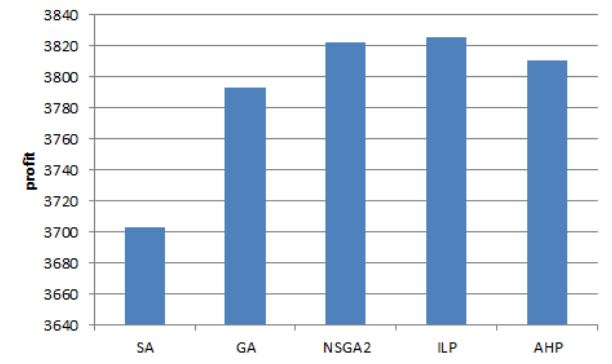
\includegraphics[width=0.9\linewidth]{bugzilla_eclipse_log(comments)_2016meancost.JPG}
\caption{ECLIPSE dataset. \normalfont{The estimated cost is 50699.70190}}
\end{subfigure}
\begin{subfigure}{\columnwidth}
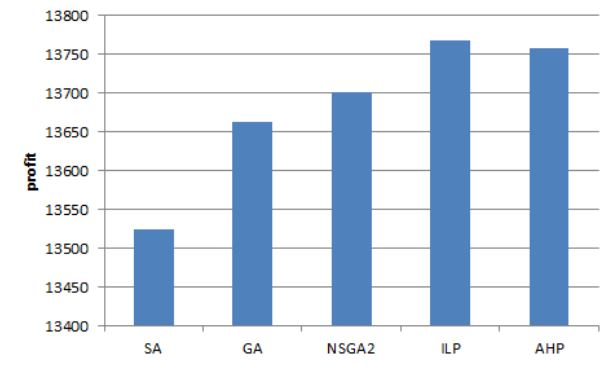
\includegraphics[width=0.9\linewidth]{bugzilla_firefox_log(comments)_2016meancost.JPG}
\caption{FIREFOX-I. \normalfont{The estimated cost is 262945.49581}}
\end{subfigure}
\begin{subfigure}{\columnwidth}
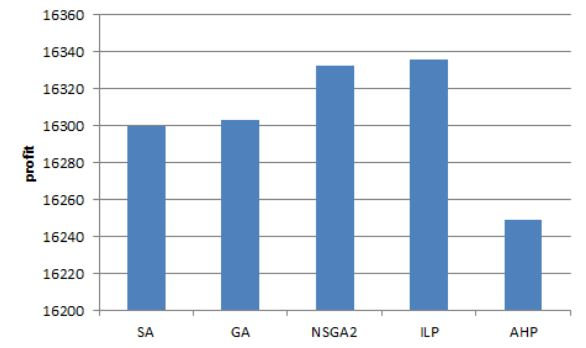
\includegraphics[width=0.9\linewidth]{bugzilla_firefox_priority_2016meancost.JPG}
\caption{FIREFOX-II. \normalfont{The estimated cost is 262945.49581}}
\end{subfigure}
\begin{subfigure}{\columnwidth}
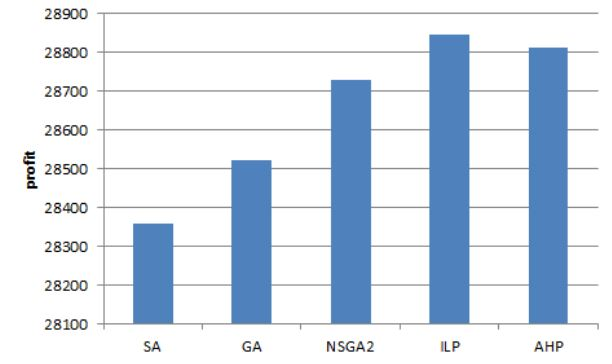
\includegraphics[width=0.9\linewidth]{bugzilla_firefox_comments-priority_2016meancost.JPG}
\caption{FIREFOX-III. \normalfont{The estimated cost is 262945.49581}}
\end{subfigure}

\caption{EX1 - Profit Comparison for each dataset}
\label{fig:DatasetProfit}
\end{figure*}


%\begin{figure*}[h]
%\begin{subfigure}{\columnwidth}
%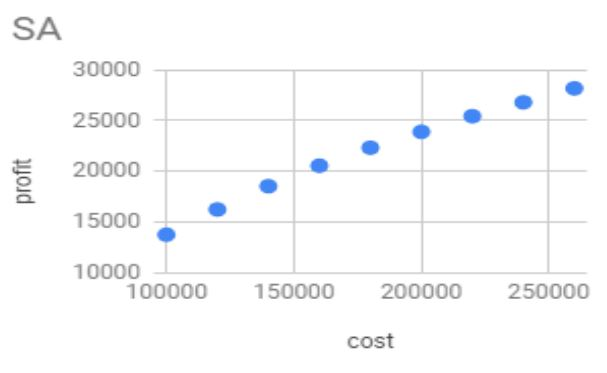
\includegraphics[width=0.9\linewidth]{SA-correlation.JPG}
%\caption{SA}
%\label{fig:subim5}
%\end{subfigure}
%\begin{subfigure}{\columnwidth}
%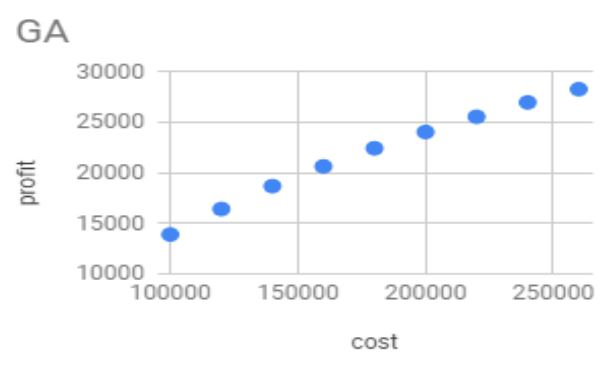
\includegraphics[width=0.9\linewidth]{GA-correlation.JPG}
%\caption{GA}
%\label{fig:subim6}
%\end{subfigure}
%\begin{subfigure}{\columnwidth}
%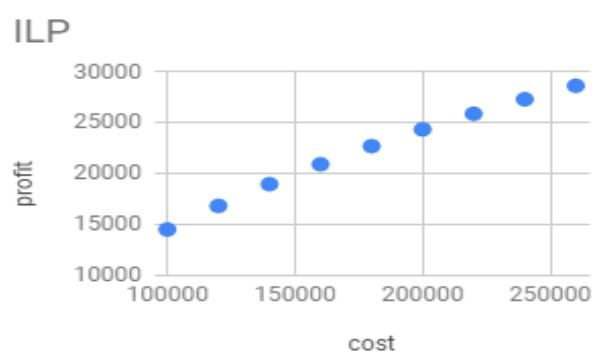
\includegraphics[width=0.9\linewidth]{ILP-correlation.JPG}
%\caption{ILP}
%\label{fig:subim7}
%\end{subfigure}
%\begin{subfigure}{\columnwidth}
%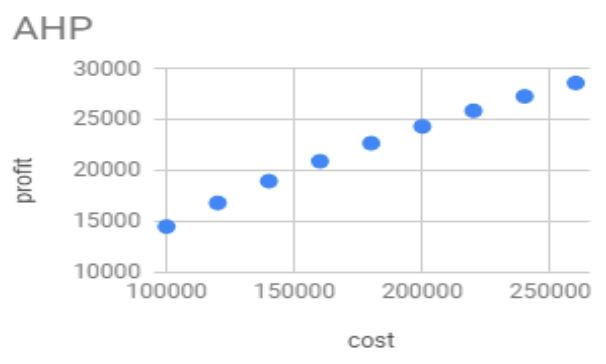
\includegraphics[width=0.9\linewidth]{AHP-correlation.JPG}
%\caption{AHP}
%\label{fig:subim8}
%\end{subfigure}

%\caption{Cost-Profit Correlation}
%\label{fig:image2}
%\end{figure*}



%\begin{figure*}[h]
%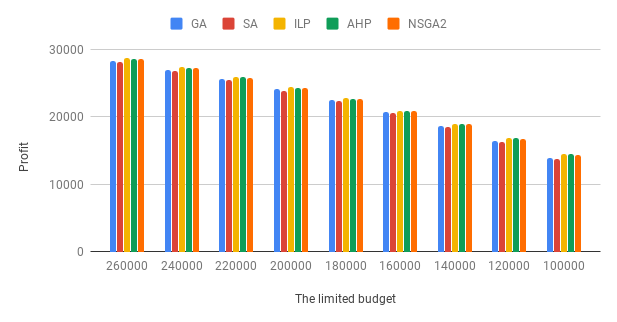
\includegraphics[width=0.9\linewidth]{ParetoFronts.png}
%\caption{Cost-Profit Correlation in one graph}
%\label{fig:paretofronts}
%\end{figure*}


\section{Experiments}
In this section, we describe what research questions were set and what experiments were performed to answer them. We used four datasets(\textit{ECLIPSE, FIREFOX-I, FIREFOX-II} and \textit{FIREFOX-III}) from Bugzilla on experiments which were described in \textbf{section 4}.

\subsection{Research Questions}

The experiments we conducted aim at answering the following research questions:\\
 
\textbf{RQ3} \textit{Which algorithms are well-suited for our datasets?}

\textbf{RQ4} \textit{Could the different profit strategy affect the performance of algorithm?}

At first experiment(EX1), we applied each algorithm to four datasets in order to compare their performances. And we hope to know the effect by different profit strategies through analyzing \textit{FIREFOX-I}, \textit{FIREFOX-II}, and \textit{FIREFOX-III} dataset which are based on FIRFOX dataset but has a different profit strategy.\\

\textbf{RQ5} \textit{What is the correlation between cost and profit?}

At second experiment(EX2), we applied each algorithm to \textit{FIREFOX-III} dataset to see the correlation between cost and profit under the real estimated cost. And also, we expected to get the interesting range which have a great change as the limited budget are increased or decreased. For example, let's assume $R = {r_1, r_2, \ldots, r_5}$, $Cost = {10, 9, 8, 2, 1}$ and $Profit = {10, 9, 8, 2, 1}$. Then, if we see the maximum profit while decreasing the limited budget, we can verify that there is a peculiar point which have a great change of profit when the limited budget is 7. So, if possible, we wanted to verify a peculiar part on EX2.
\\

\textbf{RQ6} \textit{Which algorithm and profit strategy are more similar to the real dataset?}

To identify how much our solution are similar to the real world, at third experiment(EX3), we compared the similarity between the real resolved set and the decision vector which is a result of each algorithms.

\subsection{Experimental set up}
All heuristic approaches(SA, GA and NSGA-II) were run for 500,000 function evaluations. SA started from a greedy solution and GA and NSGA-II started from the initial population which contains a greedy solution. The population size was set to 200. So each experimental execution of GA and NSGA-II was terminated when the generation number reached 2,500. GA and NSGA-II used the tournament selection(tournament size is 5), single-point cross-over, and bit-wise mutation for binary-coded GAs. The cross-over probability and the mutation probability were set to 0.8 and 1/N (where N is the length of chromosome same with the number of requirements). Every heuristic algorithms were executed 3 times for each experiment.



\section{Result and Analysis}
All results of heuristic algorithms are averaged.\\

\textbf{RQ3}\textit{Which algorithms are well-suited for our datasets?}

At EX1, we applied two deterministic and three heuristic algorithms to four datasets and compared the averaged maximum profit to each other. Figure \ref{fig:DatasetProfit} shows the results of EX1. Each graph expresses the profit of five algorithms under the limited budget(= the estimated cost).

In these results, the profit of each algorithm were bigger than the real profit in Table \ref{table:Dataset}. And, in every case, the ILP has the biggest profit. However, the order of other algorithms are slightly changed for dataset.

The SA has the smallest profit in most cases, except Figure \ref{fig:DatasetProfit}-(c). Although the SA started from a greedy solution, there is little difference between the result and a greedy solution. The profit of GA is bigger than SA and smaller than NSGA-II in every cases. So, the profit is high in order of NSGA-II, GA, then SA. The AHP has good performances for some cases. However, it has the lowest profit in \ref{fig:DatasetProfit}-(c).

The run time is also critical point to evaluate the performance. The run time of two deterministic algorithms takes just a few seconds. However, the run time of three heuristic algorithms takes more than 10 minutes. Although we consider that ILP used ILP solver, the run time of deterministic algorithms were much faster than heuristic algorithms.

Therefore, we can conclude that the ILP is well-suited for our datasets and also it is much faster than other heuristic algorithms.\\


\textbf{RQ4} \textit{Could the different profit strategy affect the performance of algorithm?}

To see the effect of different profit strategy, let's see the figure \ref{fig:DatasetProfit}-(b), (c), and (d) which are based on FIREFOX dataset but each of them has a different profit strategy. In the figure \ref{fig:DatasetProfit}-(b) and (d), GA has much bigger profit than SA and AHP has good performances enough to exceed NSGA-II. However, In the figure \ref{fig:DatasetProfit}-(c), GA has just little improvement from a greedy solution and AHP has the lowest profit among all algorithms. Therefore, we identified that the different profit strategy can affect the performance of algorithms.\\

\textbf{RQ5} \textit{What is the correlation between cost and profit?}

At EX2, we got the profits while changing the cost constraint. The result is expressed in Table \ref{table:ParetoFront}. In the results, profits of each algorithms are all increasing almost similarly and the order of profits(ILP, AHP. NSGA-II, GA, then SA) are same in every case. And also, we observed that the change of profits become smaller as the limited budget increases.

One of the reasons to perform EX2 was that we wondered if there is a peculiar part in cost-profit graph. However, we cannot observe prominently peculiar part on EX2.\\


\textbf{RQ6} \textit{Which algorithm and profit strategy are more similar to the real dataset?}

%At first experiment, we applied five algorithms to four datasets and compared the maximum profit each other. In \textbf{Table \ref{table:DatasetProfit}}, upper two rows are estimated cost sum and real profit sum of each datasets. Below these rows, there are averaged profits for each algorithms on four datasets. At the result, every profits for algorithms are bigger than real profit sum. Also, consumed time to return maximum profit was exceedingly short in ILP and AHP, rather than SA, GA, and NSGA-II.

%\textbf{Figure \ref{fig:DatasetProfit}} is the graphs of \textbf{table 1}. Each graph %expresses the averaged profit of five algorithms. At the result, the profit of ILP is %the biggest, and the profit of NSGA-II and AHP is bigger than SA and GA in most case. %Except ILP and AHP, maximum profit is high in order of NSGA-II, GA, then SA.

%At experiment 2, we got the profits while changing the cost constraint. The result is expressed in \textbf{Figure \ref{fig:paretofronts}}. \textbf{Figure \ref{fig:paretofronts}} expresses maximum profits on each cost, and \textbf{Figure 3} is integrating graph of \textbf{Figure 2} because of comparing the difference for four algorithms.

%The result is that they are all increasing almost similarly. One of the reasons to perform this experiment was that we wondered if there is a peculiar part in cost-profit graph.(if there is exceeding increase in profit) And at the result, there is no prominently peculiar part, and all the results are increasing normally.

\begin{table*}[t]
\caption{EX2 - Profit on each limited budget}
\begin{tabular}{@{}crrrrr@{}}
\toprule
\multicolumn{1}{c}{\multirow{2}{*}{\begin{tabular}[c]{@{}c@{}}The limited\\ budget\end{tabular}}} & \multicolumn{5}{c}{Algorithms}                                                                                                    \\ \cmidrule(l){2-6} 
\multicolumn{1}{c}{}                                                                              & \multicolumn{1}{c}{AHP} & \multicolumn{1}{c}{ILP} & \multicolumn{1}{c}{SA} & \multicolumn{1}{c}{GA} & \multicolumn{1}{c}{NSGA-II} \\ \midrule
100,000 & 14472.21303& \textbf{14530.92923}& 13787.94014& 13916.62496& 14359.51809\\
120,000 & 16798.95935& \textbf{16845.48739}& 16269.28033& 16440.60658& 16746.14339\\
140,000 & 18948.34660& \textbf{18979.35023}& 18553.36746& 18706.04924& 18906.95215\\
160,000 & 20906.31785& \textbf{20934.94744}& 20559.69749& 20656.69427& 20873.08535\\
180,000 & 22683.10701& \textbf{22718.92665}& 22332.52554& 22449.04724& 22651.51132\\
200,000 & 24343.18852& \textbf{24369.86106}& 23894.25792& 24054.60654& 24281.04096\\
220,000 & 25881.18360& \textbf{25901.23028}& 25425.18545& 25565.45349& 25804.51079\\
240,000 & 27305.09756& \textbf{27324.51067}& 26790.58789& 26987.08126& 27214.27095\\
260,000 & 28626.58769& \textbf{28653.54334}& 28161.56720& 28293.21833& 28556.63614\\ \bottomrule
\end{tabular}
\label{table:ParetoFront}
\end{table*}
\begin{figure*}[h]
\centering
  \begin{subfigure}[b]{0.95\linewidth}
    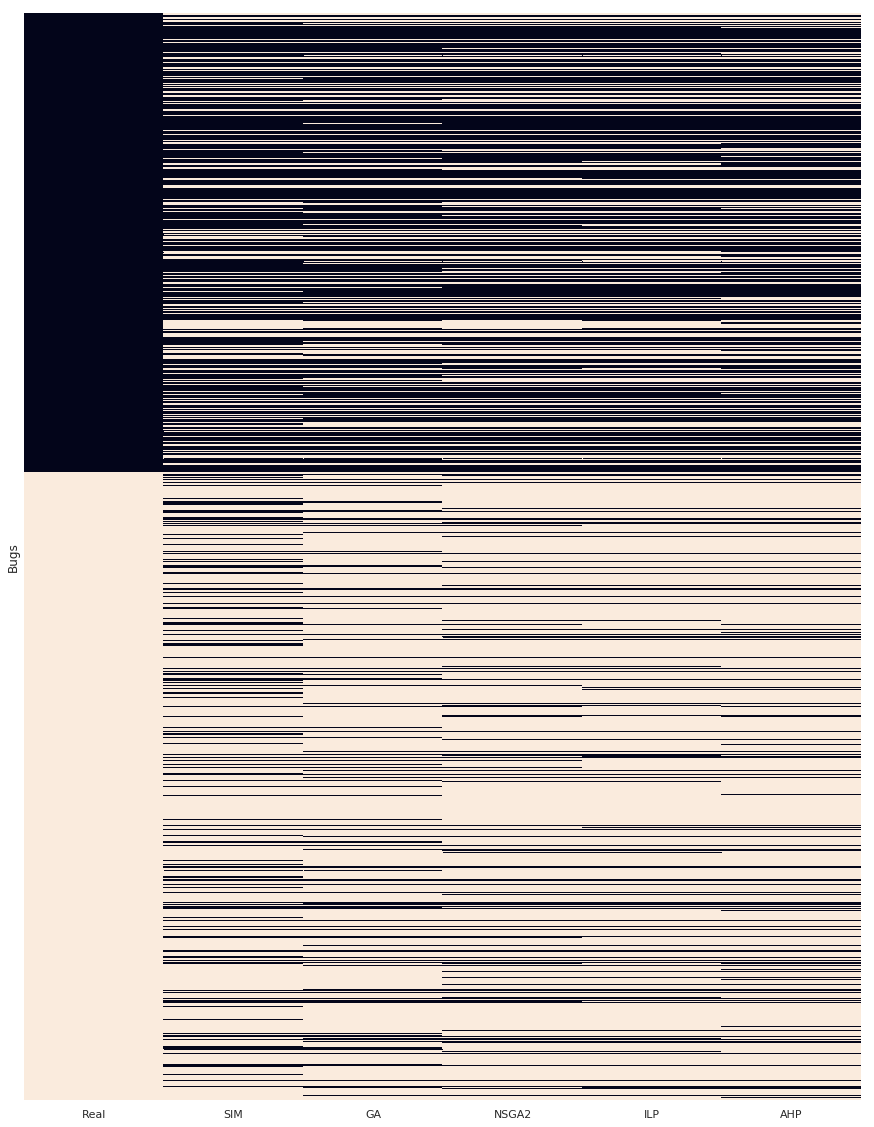
\includegraphics[width=\linewidth]{images/heatmap_ec.png}
  \end{subfigure}
  \caption{Requirements Heatmap in Eclipse Repositories(white = selected, Black = unselected)}
  \label{fig:time_cost}
\end{figure*}

\section{Conclusion}
The research question we presented was two things.
The RQ1. "Could we estimate profit from Bugzilla without forward looking?". We were able to get a proposal for the demand of custmers in Bugzilla through Priority and Comment. The RQ2. "Could we estimate profit from Bugzilla without forward looking?". We define the Cost in Bugzilla as time. The component's Cost is not accurate. However, the costs are not meaningless given the trends of 2016 and 2017. With this research question, we have built a dataset in the real world for NRP research.

In the results of the experiment.
EX1. was profit comparison. Exept for dataset with priority, the ILP has the highest result. And deterministic algorithms that AHP and ILP are very fast than heuristic algorithms. And Ex1 can answer RQ3 and RQ4. Ex2. is a comparison of the results of the profit according to the cost limit. As we mentioned, we found that limits of the Cost and the Profit had a linear relationship, regardless of algorithm. but it doesn't seem have much meaning. In RQ6. The result of algorithms were similar to those actual selection. These results show that tere are no major problems with applying NRP argorithms to our dataset. Therefore, the dataset was well set to solve the NRP.

In previous NRP studies, both dataset were applied with the random Cost and Profit values. But our project use actual situations value. It also showed that the NRP's algorithm worked well. In this way, later NRP studies have shown the possibility of using real situations rather than random values. 


